\chapter{Il Protocollo}
\label{chap:protocollo}

In questo capitolo verrà trattato il protocollo proposto per l'implementazione
della Timed-Release Encryption sui DLT.
Cercheremo di spiegare
l'idea che sta alla base con l'ausilio di un esempio.

Rientra nella categoria degli approcci
con \textit{trusted agents} (si veda \ref{subsec:trusted-agents}).
L'idea è quella di distribuire agli agenti gli \textit{share} del messaggio
e sfruttare alcuni smart contract per
fornire loro degli incentivi economici affinché pubblichino lo share
loro assegnato una volta raggiunta la deadline.
La blockchain viene utilizzata come orologio di riferimento
per capire se la deadline è stata raggiunta.

\section{Versione base}
\label{sec:versione-base}
Immaginiamo che Carol abbia bisogno di Timed-Release Encryption su un certo messaggio $ x $.
Per farlo decide farsi aiutare da Alice. Quest'ultima
impegna a conservare il messaggio e a renderlo pubblico solo dopo un
certo istante di tempo $ \tau $.
Diremo che Carol è il \textit{client} e che Alice è l'\textit{agent}.

Alice vuole essere retribuita per la conservazione di $ x $. Viene quindi fissata
una ricompensa \textit{prize}. Chiaramente Alice vuole essere sicura di
ottenere la ricompensa se rispetta il suo impegno. Allo stesso tempo Carol
vuole avere la certezza che Alice possa riscattare il premio solo se si comporta
in maniera corretta.
Carol inoltre non vuole che soggetti terzi partecipino all'accordo, perché desidera
che sia $ x $ sia l'accordo stesso rimangano segreti.
Per ottenere ciò decidono di usare uno smart contract.

\paragraph{Inizializzazione}
Nella fase iniziale Carol comunica il messaggio $ x $ ad Alice. Allo stesso tempo invia
allo smart contract una certa cifra in criptomoneta
che corrispone alla somma tra il \textit{prize} da corrispondere ad Alice e un
\textit{pawn} che le verrà restituito al termine delle operazioni, un hash
crittografico del messaggio $ x $, l'istante di tempo $ \tau $ e una tolleranza $ \delta $.

\begin{figure}[H]
	\centering
	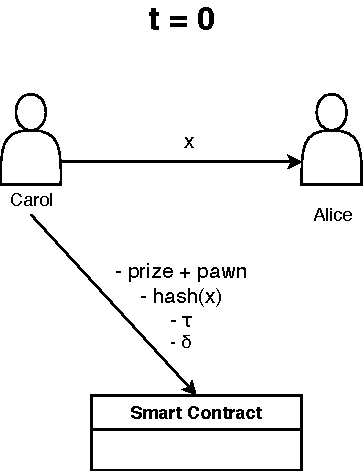
\includegraphics[width=0.3\linewidth]{images/chap_protocollo/base-creazione.pdf}
	\caption{Inizializzazione (versione base)}
\end{figure}

\paragraph{Pubblicazione}
Alice conserva quindi $ x $ e lo rende noto al tempo $ t^{*} $
(con $ \tau \leq t^{*} \leq \tau + \delta $).\footnote{Il $ \delta $ serve a far si che
	Alice pubblichi puntualmente il messaggio. Se non ci fosse questo vincolo temporale
	potrebbe rilasciare il messaggio anche con molto ritardo rispetto a
	$ \tau $ ed ottenere comunque
	la ricompensa.}
Per farlo invia allo smart contract il messaggio $ x $,
ed in cambio ottiene il suo \textit{prize}.
Allo stesso tempo, Alice riottiene il \textit{pawn} che aveva versato in precedenza.
\footnote{Ad una prima analisi può sembrare che il \textit{pawn} sia inutile,
	ma in realtà è necessario per proteggersi da alcuni tipi di attacchi.
	Le ragioni dettagliate verranno discusse nel capitolo \ref{chap:analisi-robustezza}.
	TODO sistemare}
\begin{figure}[H]
	\centering
	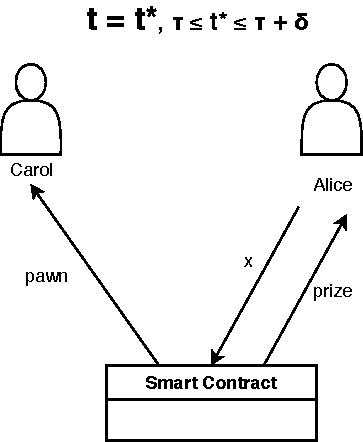
\includegraphics[width=0.3\linewidth]{images/chap_protocollo/base-pubblicazione.pdf}
	\caption{Pubblicazione del messaggio (versione base)}
\end{figure}

\paragraph{Lettura del messaggio}
Dopo il tempo $ t^{*} $, ossia dopo che Alice ha inviato $ x $ allo smart contract,
il messaggio diventa pubblico e
chiunque può leggerlo.
\begin{figure}[H]
	\centering
	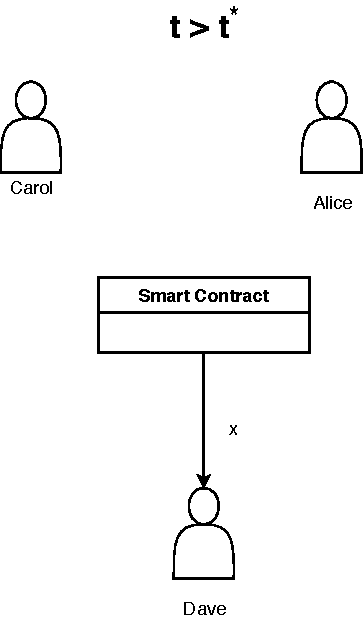
\includegraphics[width=0.27\linewidth]{images/chap_protocollo/base-leggi.pdf}
	\caption{Lettura del messaggio (versione base)}
\end{figure}

\paragraph{Pubblicazione anticipata}
Cosa succede se Alice prova a riscattare il premio prima dell'istante $ \tau $?
Semplicemente lo smart contract rifiuta la sua richiesta.
\begin{figure}[H]
	\centering
	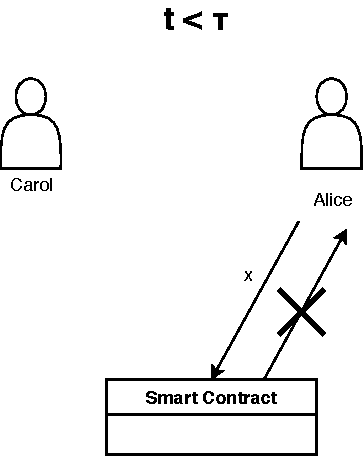
\includegraphics[width=0.3\linewidth]{images/chap_protocollo/base-anticipo.pdf}
	\caption{Tentativo di pubblicazione anticipata (versione base)}
\end{figure}

\paragraph{Leak}
E se Alice cede (volontariamente o a causa di un furto)
il segreto ad Eve prima del tempo $ \tau $?
In questo caso Eve può usare $ x $ per ottenere una ricompensa
\textit{counterprize} \footnote{dove \textit{counterprize} $ \ll $ \textit{prize}.
	Le ragioni di questo vincolo sono spiegate al capitolo \ref{chap:analisi-robustezza}.}
Il riscatto del \textit{counterprize} impedisce ad Alice di ottenere il suo premio.
È evidente che l'interesse di Alice è quello di mantenere $ x $ segreto.
\begin{figure}[H]
	\begin{minipage}{0.4\textwidth}
		\centering
		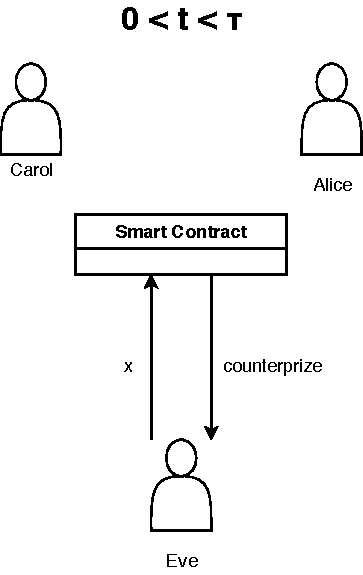
\includegraphics[width=.7\linewidth]{images/chap_protocollo/base-leak-1.pdf}
		\caption{Riscatto del counterprize (versione base)}
	\end{minipage}\hfill
	\begin{minipage}{0.4\textwidth}
		\centering
		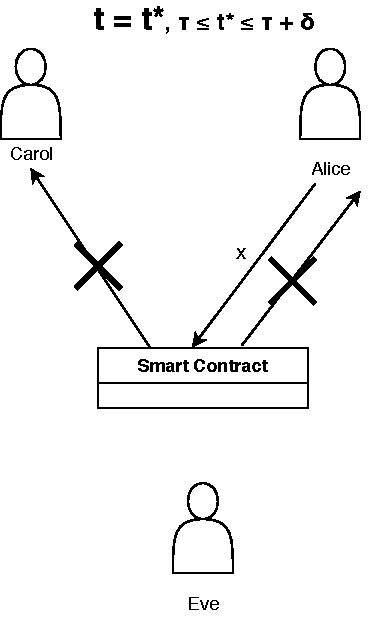
\includegraphics[width=.7\linewidth]{images/chap_protocollo/base-leak-2.pdf}
		\caption{Impossibilità di riscatto del prize (versione base)}
	\end{minipage}
\end{figure}

\section{Versione avanzata}
Facciamo notare che nella versione base
Alice conosce sin
dall'inizio il messaggio
$ x $, perché le è stato affidato nella prima fase del processo.
Ma se Carol volesse che il messaggio rimanga segreto anche ad Alice?
Per soddisfare questa condizione Alice ha bisogno di (almeno) un altro agente,
Bob, e di un
algoritmo di \textit{secret sharing}\footnote{Un algoritmo di secret sharing
	è un algoritmo che permette di
	distribuire un certo segreto tra un gruppo di $ n $ partecipanti, ad ognuno dei quali viene
	assegnato uno \textit{share}. Il segreto può essere ricostruito solo unendo un numero di share
	pari ad un fissato threshold $ t $.}.

\paragraph{Inizializzazione}
Alice, utilizzando un algoritmo di secret sharing, ottiene due share
$ x_A $ e $ x_B $. Invia questi share rispettivamente ad Alice e a Bob ed inizializza
lo smart contract versando due \textit{prize} e due \textit{pawn},
inviando gli hash crittografici
degli share, il tempo $ \tau $ e la tolleranza $ \delta $.
\begin{figure}[H]
	\centering
	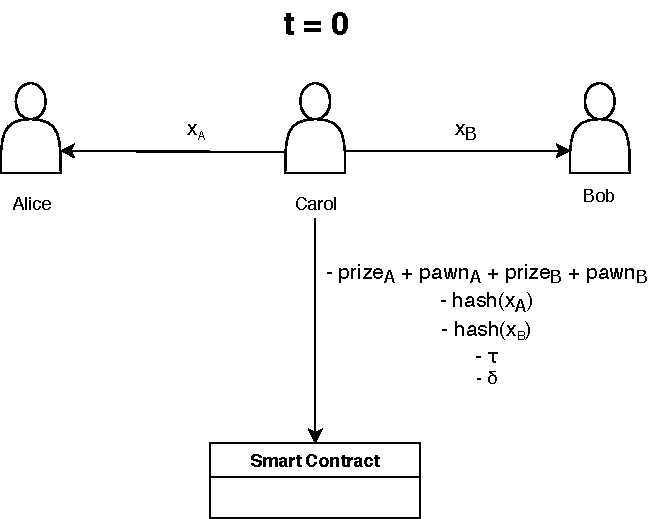
\includegraphics[width=0.6\linewidth]{images/chap_protocollo/avanzato-creazione.pdf}
	\caption{Inizializzazione (Versione avanzata)}
\end{figure}



\paragraph{Pubblicazione}
Alice e Bob pubblicano i loro share rispettivamente al tempo $ t^*_A $ e $ t^*_B $
(con $ \tau \leq t^*_A \leq \tau + \delta $, $ \tau \leq t^*_B \leq \tau + \delta $).
In cambio ottengono i loro
\textit{prize}.
Allo stesso tempo Alice riottiene i rispettivi \textit{pawn} che aveva versato
in precedenza.
\begin{figure}[H]
	\begin{minipage}{0.45\textwidth}
		\centering
		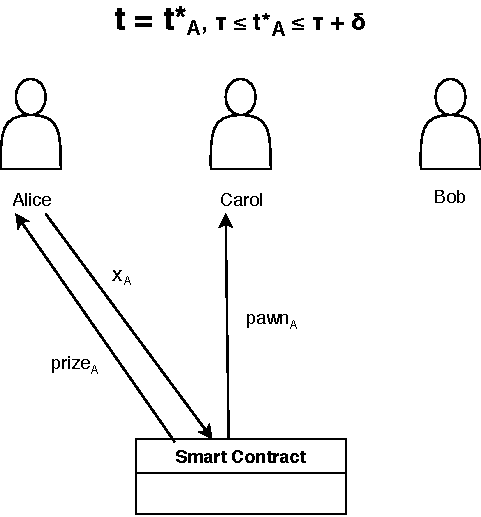
\includegraphics[width=.7\linewidth]{images/chap_protocollo/avanzato-pubblicazione-a.pdf}
		\caption{Pubblicazione dello share $ x_A $ (versione avanzata)}
	\end{minipage}\hfill
	\begin{minipage}{0.45\textwidth}
		\centering
		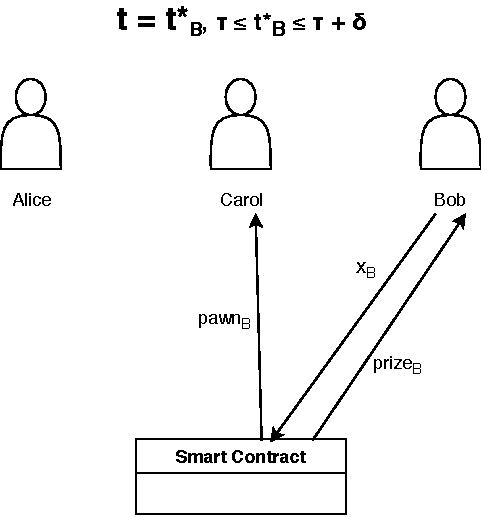
\includegraphics[width=.7\linewidth]{images/chap_protocollo/avanzato-pubblicazione-b.pdf}
		\caption{Pubblicazione dello share $ x_B $ (versione avanzata)}
	\end{minipage}
\end{figure}

\paragraph{Accesso al messaggio}
Dopo il tempo $ t^* = max(t^*_A, t^*_B) $, ossia dopo che sia Alice sia Bob
hanno inviato $ x_A $ ed $ x_B $
allo smart contract, chiunque può leggere gli share dallo smart contract e quindi
ricostruire il messaggio $ x $.
\begin{figure}[H]
	\centering
	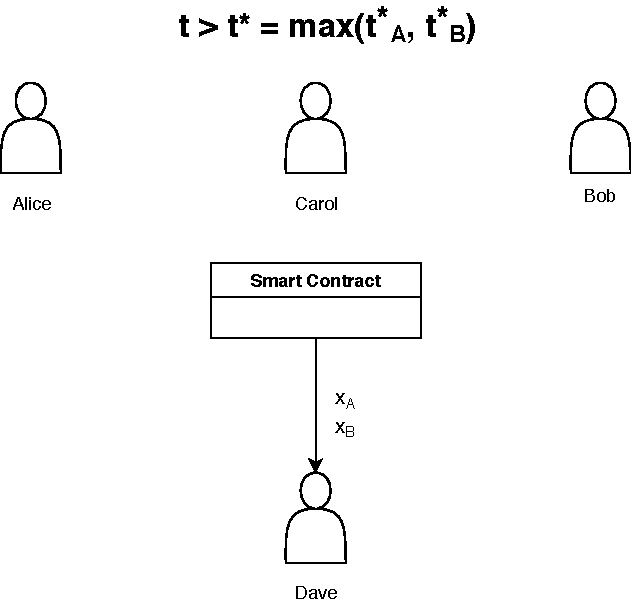
\includegraphics[width=0.5\linewidth]{images/chap_protocollo/avanzato-leggi.pdf}
	\caption{Lettura del messaggio (versione avanzata)}
\end{figure}

\paragraph{Leak}
Cosa succede se Bob cede il suo share ad Eve prima del tempo $ \tau $?
Anche in questo caso Eve può usare $ x_B $ per ottenere una ricompensa
\textit{counterprize}.
Il riscatto del \textit{counterprize} impedisce a Bob di ottenere il suo premio.
Da notare che se Alice si comporta in maniera corretta, ossia se tiene segreto il
suo share, è in grado di ottenere la sua ricompensa indipendentemente dal comportamento
di Bob.
\begin{figure}[H]
	\centering
	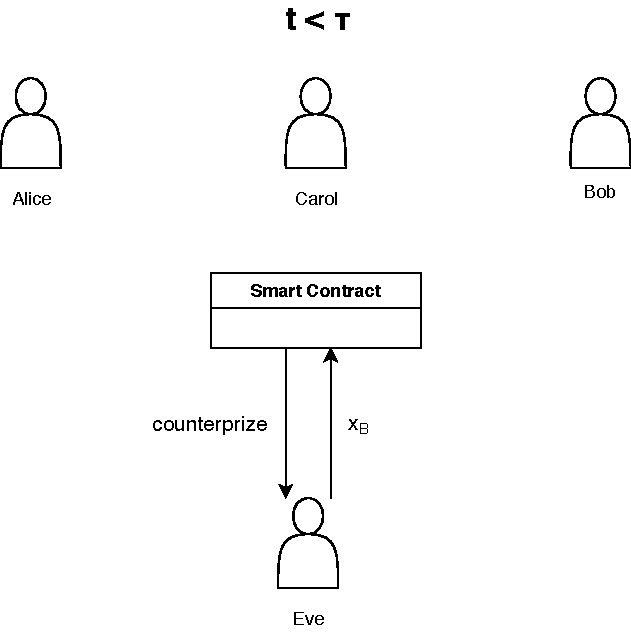
\includegraphics[width=0.4\linewidth]{images/chap_protocollo/avanzato-leak-1.pdf}
	\caption{Riscatto del counterprize (versione avanzata)}
\end{figure}

\begin{figure}[H]
	\begin{minipage}{0.45\textwidth}
		\centering
		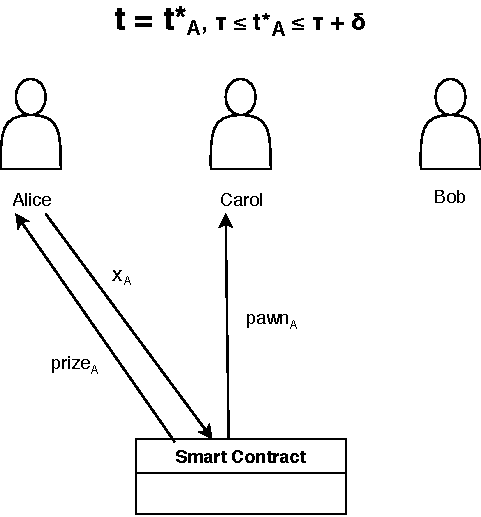
\includegraphics[width=.8\linewidth]{images/chap_protocollo/avanzato-leak-2-a.pdf}
		\caption{Riscatto di $ \text{prize}_A $ (versione avanzata)}
	\end{minipage}\hfill
	\begin{minipage}{0.45\textwidth}
		\centering
		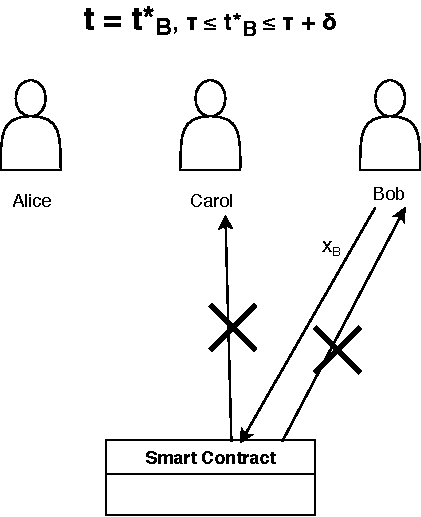
\includegraphics[width=.71\linewidth]{images/chap_protocollo/avanzato-leak-2-b.pdf}
		\caption{Impossibilità di riscatto di $ \text{prize}_B $ (versione avanzata)}
	\end{minipage}
\end{figure}

Abbiamo visto un esempio con la partecipazione di due agenti,
ma il protocollo
può essere analogamente implementato con un numero qualsiasi $ N $ di agenti.


\section{Varianti}
\subsection{Invio del messaggio solo a determinati attori}
Dopo il tempo $ t^* $ il messaggio diventa pubblico a chiunque abbia accesso
allo smart contract. In alcuni contesti questo potrebbe essere un problema, perché
potremmo volere che il messaggio possa essere letto solo da determinati attori.

Una possibile soluzione è aggiungere un layer di cifratura simmetrica al messaggio
prima di criptarlo con la TRE.
La procedura è la seguente.
Per prima cosa si cripta il messaggio $ m $ con cifratura simmetrica e chiave $ k $
ottenendo $ m^\prime $. Allo stesso tempo per ogni account destinatario designato
$ A_1, ..., A_n $ si generano $ k_1, ..., k_n $, dove ogni $ k_i $ è $ k $ cifrato con la
chiave pubblica del portafoglio $ A_i $. A questo punto si genera un header
$ h = (k_1, ..., k_n) $. Infine si crea $ x = (h, m^\prime) $ e lo si utilizza come
segreto per il protocollo proposto.
Una volta raggiunta la deadline $ x $ diventa pubblico, ma $ m $ no. I destinatari designati
$ A_i $ possono leggere $ m $ estraendo $ k_i $ dall'header di $ x $, ottenere
$ k $ decriptandolo con la propria chiave privata e quindi decriptare $ m^\prime $.

\subsection{Divisione di share in più livelli}
La versione avanzata del protocollo proposto può essere estesa con una divisione su più livelli
degli share distribuiti agli agenti.
L'idea è quella di creare un \textit{albero di distribuzione degli share}.
Partendo dal messaggio $ x $, che rappresenta il nodo radice, si ottengono gli share $ x_{1i} $,
rappresentati come nodi figli.
A questo punto su ogni share $ x_{1i} $ si opera nuovamente il protocollo proposto,
utilizzando questa volta $ x_{1i} $ come segreto.
Si ottengono così gli share di secondo livello $ x_{2i} $.
Si può procedere iterativamente in questo modo fino a raggiungere la profondità desiderata.
Gli share nei nodi foglia vengono poi assegnati agli agenti.
Non è strettamente necessario creare un albero bilanciato.

\begin{figure}[H]
	\centering
	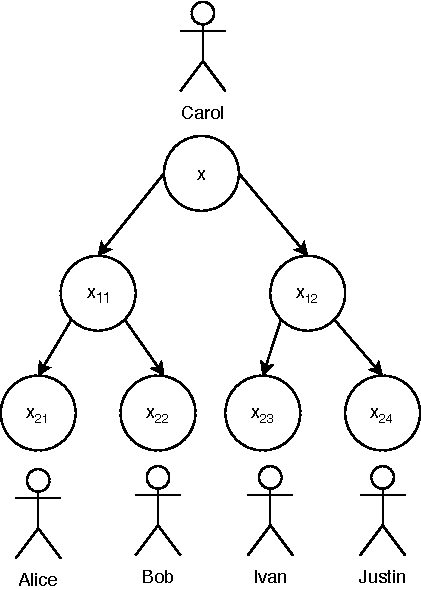
\includegraphics[width=0.45\linewidth]{images/chap_protocollo/protocollo-gerarchia.pdf}
	\caption{Esempio di un albero di distribuzione degli share}
\end{figure}

Le scelte progettuali riguardo la struttura dell'albero di distribuzione degli share hanno un
impatto sulla robustezza dell'implementazione del protocollo proposto. Per una analisi più
approfondita rimandiamo al capitolo \ref{chap:analisi-robustezza}.

\subsection{Ricompense intermedie}
Immaginiamo che Carol abbia bisogno di Timed-Release Encryption su un certo messaggio $ x $, e
che la deadline $ \tau $ sia molto avanti nel tempo.
Immaginiamo inoltre che, fissata una ricompensa \textit{prize},
l'agente Alice dia la sua disponibilità, ma a patto di non dover attendere fino al tempo $ \tau $
per riceve l'intera
ricompensa. Una soluzione è quella di prevedere delle ricompense intermedie.
Per realizzarle si procede nel modo seguente.

Il messaggio $ x $ viene diviso in $ n $ share con threshold $ t = n $.
Per ogni share si applica la versione base del protocollo
con deadline $ \tau_1, \tau_2, ... , \tau_n = \tau $
tali che $ \tau_1 < \tau_2 < ... < \tau_n = \tau $ e con rispettive ricompense
$ \textit{prize}_1, \textit{prize}_2, ..., \textit{prize}_n $ tali che
$ \textit{prize}_1 + \textit{prize}_2 +, ... + \textit{prize}_n = \textit{prize} $.
In questo modo l'agente Alice può eseguire delle pubblicazioni intermedie e ricevere le relative
ricompense; allo stesso tempo il messaggio rimarrebbe segreto fino a quando non viene pubblicato
l'ultimo share, ossia fino alla deadline $ \tau $.
Questa metodologia può essere applicata analogamente anche alla versione avanzata.